\documentclass[a4paper,12pt]{article}
\usepackage{fullpage}
\usepackage[british]{babel}
\usepackage[T1]{fontenc}
\usepackage{amsmath}
\usepackage{amssymb}
\usepackage[T1]{fontenc}
\usepackage{natbib}
\setcitestyle{square}
\usepackage[utf8]{inputenc}
%\usepackage{amsthm} \newtheorem{theorem}{Theorem}
\usepackage{color}
\usepackage{float}
\usepackage{authblk}
\usepackage{todonotes}
\usepackage{algorithmicx}
\usepackage{algpseudocode}% http://ctan.org/pkg/algorithmicx

\usepackage{caption}
\DeclareCaptionFont{white}{\color{white}}
\DeclareCaptionFormat{listing}{\colorbox{gray}{\parbox{\textwidth}{#1#2#3}}}
\captionsetup[lstlisting]{format=listing,labelfont=white,textfont=white}

\usepackage{alltt}
\usepackage{listings}
\usepackage{algorithm}
%\usepackage{algorithmicx}
\usepackage{subfig}
\lstset{% parameters for all code listings
language=Python,
frame=single,
basicstyle=\small, % nothing smaller than \footnotesize, please
tabsize=2,
numbers=left,
% framexleftmargin=2em, % extend frame to include line numbers
%xrightmargin=2em, % extra space to fit 79 characters
breaklines=true,
breakatwhitespace=true,
prebreak={/},
captionpos=b,
columns=fullflexible,
escapeinside={\#*}{\^^M}
}



\usepackage{tikz}
\usetikzlibrary{arrows}
\usetikzlibrary{automata,positioning}


\newcommand{\abpsender}[1][]{
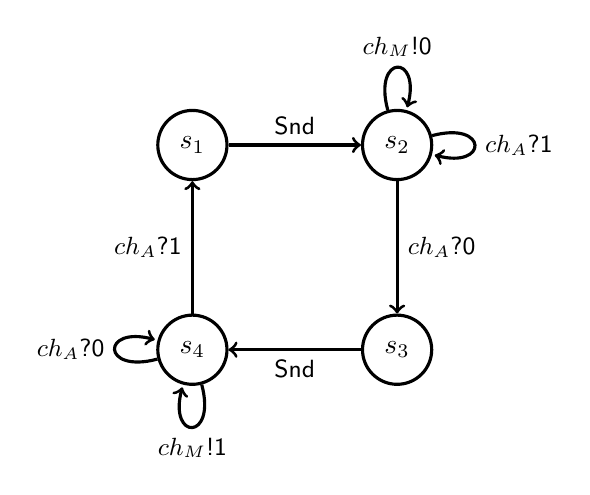
\begin{tikzpicture} [->,auto,node distance=2.6cm,line width=0.4mm]
  \node[state] (1) {$s_1$};
  \node[state] (2) [right of=1] {$s_2$};
  \node[state] (3) [below of=2] {$s_3$};
  \node[state] (4) [left of=3] {$s_4$};

  \path[every node/.style={font=\sffamily\small}]
    (1) edge node [above] {Snd} (2)
    (2) edge node [right] {$ch_A$?0} (3)
        edge [loop right] node {$ch_A$?1} (2)
        edge [loop above] node {$ch_M$!0} (2)
    (3) edge node [below] {Snd} (4)
    (4) edge node [left] {$ch_A$?1} (1)
        edge [loop left] node {$ch_A$?0} (4)
        edge [loop below] node {$ch_M$!1} (4);
\end{tikzpicture}
}

\newcommand{\abpreceiver}[1][]{
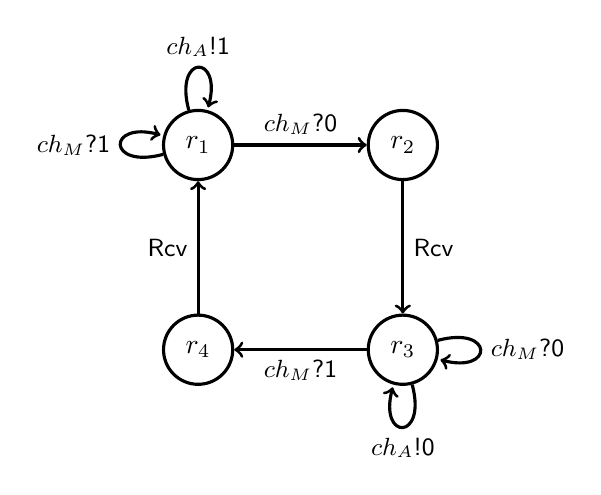
\begin{tikzpicture} [->,auto,node distance=2.6cm,line width=0.4mm]

  \node[state] (1) {$r_1$};
  \node[state] (2) [right of=1] {$r_2$};
  \node[state] (3) [below of=2] {$r_3$};
  \node[state] (4) [left of=3] {$r_4$};

  \path[every node/.style={font=\sffamily\small}]
    (1) edge node [above] {$ch_M$?0} (2)
        edge [loop left] node {$ch_M$?1} (1)
        edge [loop above] node {$ch_A$!1} (1)
    (2) edge node [right] {Rcv} (3)
    (3) edge node [below] {$ch_M$?1} (4)
        edge [loop right] node {$ch_M$?0} (3)
        edge [loop below] node {$ch_A$!0} (3)
    (4) edge node [left] {Rcv} (1);

\end{tikzpicture}
}


\newcommand{\swsender}[1][]{
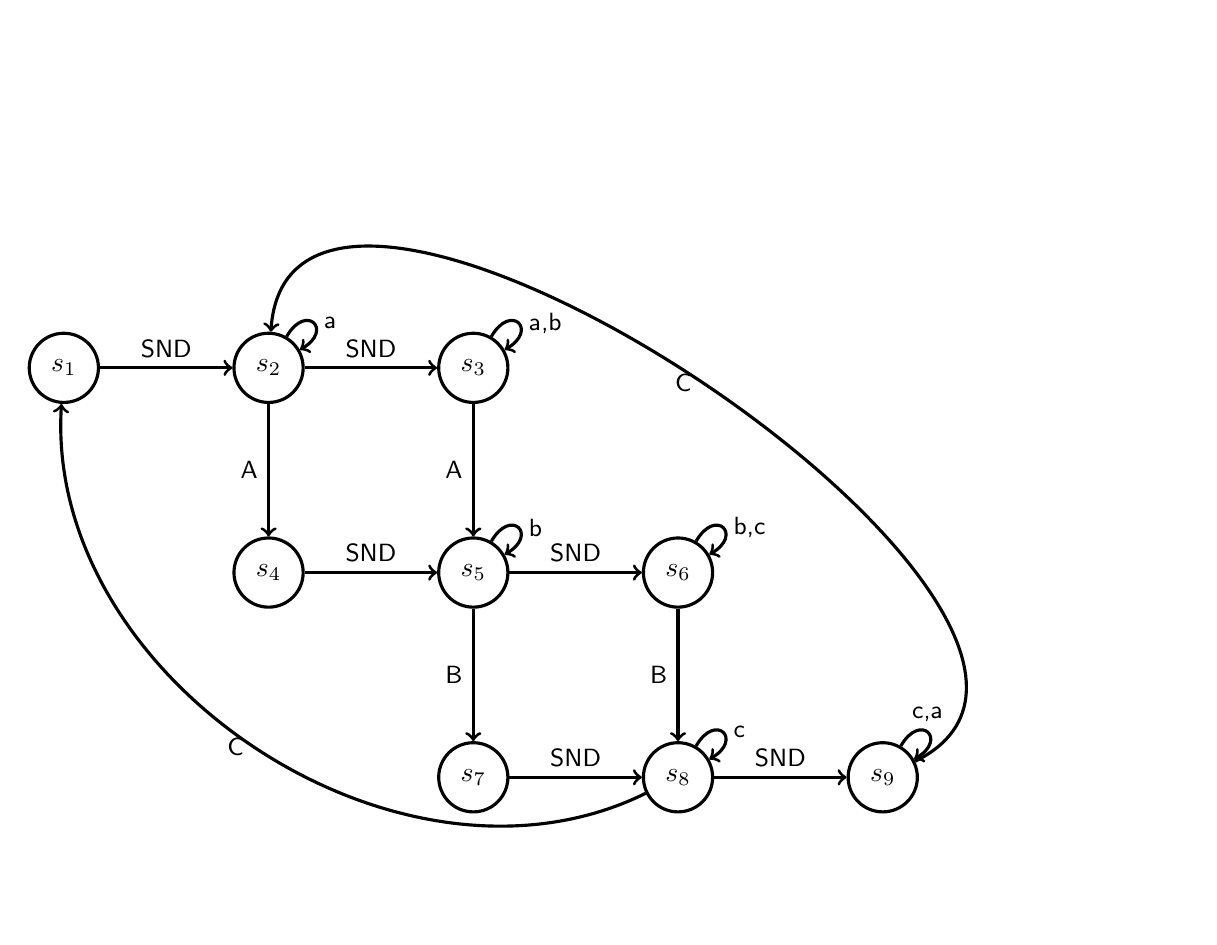
\begin{tikzpicture} [->,auto,node distance=2.6cm,line width=0.4mm]
  \node[state] (1) {$s_1$};
  \node[state] (2) [right of=1] {$s_2$};
  \node[state] (3) [right of=2] {$s_3$};
  \node[state] (4) [below of=2] {$s_4$};
  \node[state] (5) [below of=3] {$s_5$};
  \node[state] (6) [right of=5] {$s_6$};
  \node[state] (7) [below of=5] {$s_7$};
  \node[state] (8) [below of=6] {$s_8$};
  \node[state] (9) [right of=8] {$s_9$};

  \path[->,every loop/.style={in=30, out=60, looseness=3}, every node/.style={font=\sffamily\small}]
    (1) edge node [above] {SND} (2)
    (2) edge node [above] {SND} (3)
        edge [loop right] node {a} (2)
        edge node [left] {A} (4)
    (3) edge node [left] {A} (5)
        edge [loop right] node {a,b} (3)
    (4) edge node [above] {SND} (5)
    (5) edge node [above] {SND} (6)
        edge [loop right] node {b} (5)
        edge node [left] {B} (7)
    (6) edge node [left] {B} (8)
        edge [loop right] node {b,c} (6)
    (7) edge node [above] {SND} (8)
    (8) edge node [above] {SND} (9)
        edge [loop right] node {c} (8)
        edge [bend left=60] node [left] {C} (1)
    (9) edge [bend right=120] node [left] {C} (2)
        edge [loop above] node {c,a} (9);




\end{tikzpicture}
}

\newcommand{\swreceiver}[1][]{
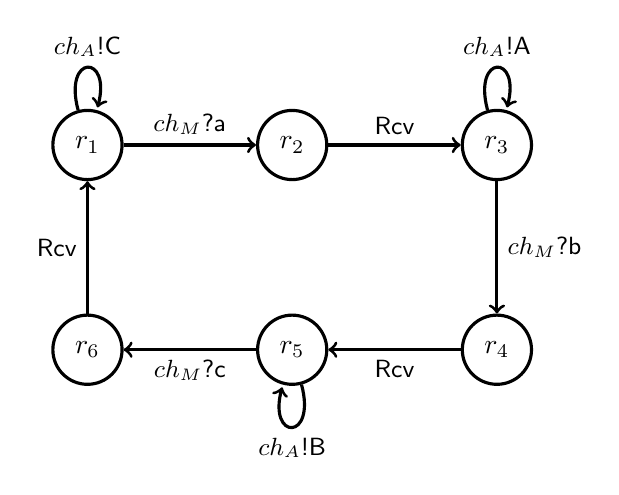
\begin{tikzpicture} [->,auto,node distance=2.6cm,line width=0.4mm]

  \node[state] (1) {$r_1$};
  \node[state] (2) [right of=1] {$r_2$};
  \node[state] (3) [right of=2] {$r_3$};
  \node[state] (4) [below of=3] {$r_4$};
  \node[state] (5) [left of=4] {$r_5$};
  \node[state] (6) [left of=5] {$r_6$};

  \path[every node/.style={font=\sffamily\small}]
    (1) edge node [above] {$ch_M$?a} (2)
  edge [loop above] node {$ch_A$!C} (1)
    (2) edge node [above] {Rcv} (3)
    (3) edge node [right] {$ch_M$?b} (4)
  edge [loop above] node {$ch_A$!A} (3)
    (4) edge node [below] {Rcv} (5)
    (5) edge node [below] {$ch_M$?c} (6)
  edge [loop below] node {$ch_A$!B} (5)
    (6) edge node [left] {Rcv} (1);

\end{tikzpicture}
}


\newcommand{\swobserver}[1][]{
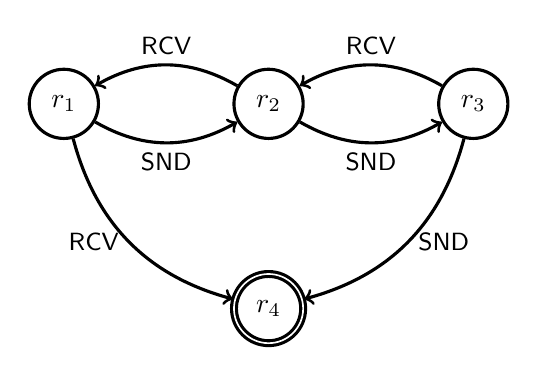
\begin{tikzpicture} [->,auto,node distance=2.6cm,line width=0.4mm]

  \node[state] (1) {$r_1$};
  \node[state] (2) [right of=1] {$r_2$};
  \node[state] (3) [right of=2] {$r_3$};
  \node[state,accepting] (4) [below of=2] {$r_4$};


  \path[every node/.style={font=\sffamily\small}]
    (1) edge [bend right] node [below] {SND} (2)
  edge [bend right] node [left] {RCV} (4)
    (2) edge [bend right] node [below] {SND} (3)
  edge [bend right] node [above] {RCV} (1)
    (3) edge [bend left] node [right] {SND} (4)
  edge [bend right] node [above] {RCV} (2); 

\end{tikzpicture}
}



\newcommand{\abpobserver}[1][]{
\begin{tikzpicture} [->,auto,node distance=2.6cm,line width=0.4mm]

%\begin{tikzpicture}[->,>=stealth',shorten >=1pt,auto,node distance=3cm,
%  thick,main node/.style={circle,fill=blue!20,draw,font=\sffamily\Large\bfseries}]

  \node[state] (1) {$o_1$};
  \node[state,accepting] (3) [right of=1] {$o_2$};
  \node[state] (2) [right of=2] {$o_3$};

  \path[every node/.style={font=\sffamily\small}]
    (1) edge [bend left] node [above] {Snd} (2)
        edge node [above] {Rcv} (3)
    (2) edge [bend left] node [below] {Rcv} (1)
        edge node [above] {Snd} (3);
\end{tikzpicture}
}

% Alter some LaTeX defaults for better treatment of figures:
    % See p.105 of "TeX Unbound" for suggested values.
    % See pp. 199-200 of Lamport's "LaTeX" book for details.
    % General parameters, for ALL pages:
    \renewcommand{\topfraction}{0.9}	% max fraction of floats at top
    \renewcommand{\bottomfraction}{0.8}	% max fraction of floats at bottom
    % Parameters for TEXT pages (not float pages):
    \setcounter{topnumber}{2}
    \setcounter{bottomnumber}{2}
    \setcounter{totalnumber}{4} % 2 may work better
    \setcounter{dbltopnumber}{2} % for 2-column pages
    \renewcommand{\dbltopfraction}{0.9}	% fit big float above 2-col. text
    \renewcommand{\textfraction}{0.07}	% allow minimal text w. figs
    % Parameters for FLOAT pages (not text pages):
    \renewcommand{\floatpagefraction}{0.7}	% require fuller float pages
% N.B.: floatpagefraction MUST be less than topfraction !!
    \renewcommand{\dblfloatpagefraction}{0.7}	% require fuller float pages

% remember to use [htp] or [htpb] for placement


\usepackage{fancyvrb}
%\DefineVerbatimEnvironment{code}{Verbatim}{fontsize=\small
%\DefineVerbatimEnvironment{example}{Verbatim}{fontsize=\small}

\usepackage{url}
\urldef{\mailsa}\path|josh0151@student.uu.se |
\urldef{\mailsb}\path|bjfo5755@student.uu.se |
\newcommand{\keywords}[1]{\par\addvspace\baselineskip
\noindent\keywordname\enspace\ignorespaces#1}


\usepackage{tikz} \usetikzlibrary{trees}
\usepackage{hyperref} % should always be the last package

% useful colours (use sparingly!):
\newcommand{\blue}[1]{{\color{blue}#1}}
\newcommand{\green}[1]{{\color{green}#1}}
\newcommand{\red}[1]{{\color{red}#1}}

% useful wrappers for algorithmic/Python notation:
\newcommand{\length}[1]{\text{len}(#1)}
\newcommand{\twodots}{\mathinner{\ldotp\ldotp}} % taken from clrscode3e.sty
\newcommand{\Oh}[1]{\mathcal{O}\left(#1\right)}

% useful (wrappers for) math symbols:
\newcommand{\Cardinality}[1]{\left\lvert#1\right\rvert}
%\newcommand{\Cardinality}[1]{\##1}
\newcommand{\Ceiling}[1]{\left\lceil#1\right\rceil}
\newcommand{\Floor}[1]{\left\lfloor#1\right\rfloor}
\newcommand{\Iff}{\Leftrightarrow}
\newcommand{\Implies}{\Rightarrow}
\newcommand{\Intersect}{\cap}
\newcommand{\Sequence}[1]{\left[#1\right]}
\newcommand{\Set}[1]{\left\{#1\right\}}
\newcommand{\SetComp}[2]{\Set{#1\SuchThat#2}}
\newcommand{\SuchThat}{\mid}
\newcommand{\Tuple}[1]{\langle#1\rangle}
\newcommand{\Union}{\cup}
\newcommand{\conf}[1]{\langle#1\rangle}
\newcommand{\subword}{\sqsubseteq}
\newcommand{\e}[1]{\emph{#1}}
\usetikzlibrary{positioning,shapes,shadows,arrows}

\usepackage{url}


\usepackage{booktabs,array}
\def\Midrule{\midrule[\heavyrulewidth]}
\newcount\rowc

\makeatletter
\def\ttabular{%
\hbox\bgroup
\let\\\cr
\valign\bgroup
\global\rowc\@ne
\hbox to 7em{\strut \hfill##\hfill}%
&&%
\global\advance\rowc\@ne
\hbox to 7em{\strut\hfill##\hfill}%
\cr}
\def\endttabular{%
\crcr\egroup\egroup}


\usepackage{amsthm}
\theoremstyle{plain}
\newtheorem{theorem}{Theorem}
\newtheorem{corollary}{Corollary}[theorem]
\newtheorem{lemma}[theorem]{Lemma}



%Specific for this document


\title{\textbf{Algorithmic Analysis of Channel machines\\ Using Small Models}}

\author{Jonathan Sharyari}
\textwidth 5.5in 
\oddsidemargin 0.5in 


\begin{document}

\maketitle


\begin{abstract}
Parameterized verification of algorithms is in general an undecidable problem, but nevertheless, solid correctness results are important in many real-life applications. It is commonly the case that such algorithms rely on unbounded buffers for their operation, communication algorithms being a typical example. Building upon abstract interpretation techniques, this project presents a verification algorithm capable of verifying the correctness of algorithms relying on unbounded \emph{lossy} buffers.

A working prototype of the algorithm was created and used to verify a number of well-known communication algorithms. The experimental results are mixed, but in most cases comparable to that of other avaiable tools for this cause, justifying further research on the topic.
\end{abstract}

\tableofcontents
\newpage
\section{Introduction}
Todays society grows more and more dependent on computer applications\todo{Do you mean I should have a reference for this?}. Often they are used directly, for example the task of paying bills online. In other cases, applications are aiding us in a more abstract manner, e.g. controlling the elevator or planning a train schedule. The common factor between the online bank, the elevator relay and the train scheduler is that the correctness of these programs is of utter importance, where program failure could have devastating results on the economy, the infrastructure or even cause harm.

This has motivated research on various techniques to find and correct potential faults, particularly in safety-critical systems. The most common technique is that of \e{testing}, i.e. observing the system behaviour on a variety of likely or even unlikely scenarios. The widespread use of testing is well-motivated, but there are several scenarios, where testing by itself is insufficient, or difficult to carry out. It would for example be costly to verify the correctness of the aforementioned elevator only by testing, as a failure could result in damages on the system.

A technique used for verification is the process of \e{simulation}. In contrast to testing, simulation can be done in an early stage of the development. Rather than first implementing an algorithm, one may simulate an abstracted model of the algorithm which may help in ensuring its correctness or find a fault in the algorithm before development has begun. An important note is that simulation techniques are not intended to be used \e{instead} of testing, but rather in combination with testing, as an abstract model of a system can never fully represent the system as a whole.

A trend in todays computing is that applications become concurrent or distributed. Such programs are inherently difficult to verify, due to the fact that although processes themselves have finite models, the results of the behaviour of asynchronous processes may be infinite. This is the case for example when the composition of a possibly infinite number of processes is observed, a common scenario when verifying  concurrent and distributed programs. Also, we are often not interested in performing verification of a \e{specific} composition of concurrent programs, but rather in verifying that it works for \e{all} compositions.

Related to this is the necessity for distributed and concurrent programs to communicate, and to do so accurately. In general, the underlying systems that we use for our communication are inreliable, in that message loss or message corruption may occur. This happens due to a variety of reasons, may that be faults in the communication links, relays or the communicating parties themselves. To overcome this problem, communication protocols are designed to be resistent to such faults, and ensuring the correctness of these protocols is paramount when ensuring reliable communication. Even when the number of communicating processes is finite, communication protocols commonly result in infinte models, as the number of sent messages may be unbounded, and there may be an infinite number of orderings thereof. The verification of such systems, which rely on communication channels, is the focus of this thesis.

The goal of \e{model checking} is to formally verify the correctness of concurrent programs with respect  to a given specification. In general, given a model of a system and a specification of its intended properties, the task is to decide whether a model meets its specification or not.

Different representations of models and properties have been proposed, as well as techniques to perform the verification. One of the most successful and most common methods is that of \e{temporal logic model checking}. Traditionally, the model is expressed as a finite state machine and the properties as propositional logic formulae. Several verification methods for such models have been proposed\cite{mcmillan1993symbolic} and although these methods have been applied to infinite models\cite{705644}, the focus has in large been on the verification of finite models.

Another approach is taken by \cite{parosh}, in which the verification of \e{parameterized systems} is attempted. \e{Parameterized systems} are systems composed of a set of processes, where the number of processes is itself a parameter of the system. This is often the case when discussing concurrent and distributed programs. Although an undecidable problem, there are methods that can provide approximation techniques that allows us to reduce the verification task to the finite state case. These methods include \e{counter abstraction techniques}\cite{counterabstraction} and \e{invisible invariant} generation\cite{invinv}. 

In \cite{parosh}, the authors take advantage of the \e{small model property} -- if a small instance of a system is enough to exhibit the relevant behaviour of the system as a whole, that instance is a small model of the system\todo[inline]{Didn't understand the comment regarding this}. An important contribution of \cite{parosh} is that they show that this property holds for \e{quasi well-ordered systems}\cite{abdulla2010} (i.e. transitions systems monotonic with respect to a well-quasi ordering)\todo[inline]{is this good enough, or did I just explain it in a circle?}, and indicates its use for yet larger sets of systems.

Using well-known techniques of \e{abstract interpretation} combined with the idea of small models, \cite{parosh} shows that parameterized systems can in fact be reduced to finite and decidable approximations of the system, and a prototype implementation of the technique substantiates this claim by empirical results.

This essay draws the attention towards systems relying on communications over asynchronous unbounded buffers. This scenario is common in communication protocols using channels and in distributed computing\cite{fredlund2007mcerlang}. An important note is that channel systems working on \e{perfect channels} are Turing powerful\todo[inline]{Why powerful and not complete? difference?}, and therefore undecidable, but it has been shown that verification of safety properties of channel systems over \e{lossy channels}, i.e. channels that may nondeterministicly lose messages, is decidable\cite{287591}\cite{gordon}. Channels systems need not only represent communication protocols, but may also be used to described other types of programs, such as cache coherence protocols and sensor systems\cite{zuck2004}.

Inspired by \cite{parosh}, I explore the possibility of using abstract interpretation techniques and small models for systems with unbounded buffers, keeping the number of programs constant. We developed a verification technique for this purpose and the resulting model was implemented and tested. 

%As previously mentioned, this is an undecidable problem in general, and this paper does \e{not} investigate exactly what class of systems that are decidable. The experimental results show that several well-known communication protocols are indeed in the scope of the tool.

%% Is this actually a decidable problem?

\paragraph{Reading this paper} Section \ref{notation} introduces some of the terminology and notation used in this paper, whereas section \ref{definitions} contains formal definitions to some of the key concepts -- these are previously known concepts, asides from their adaption to the specific context of this thesis. Section \ref{model} introduces the concepts of small models and abstract interpretation, and relates these to buffer channels to create the theoretical model for this paper. Section \ref{extensions} introduces some extensions to this model, allowing for a wider variety of modeling scenarios. In section \ref{implementation}, some abstractions and techniques are explained that allow for an efficient implementation of the verification algorithm. Further a protocol specification language is explained, that allows a user to define and use the verification tool without knowledge of the intricacies of the internal model. The results of the verifier when applied to a number of well-known communication algorithms is presented in section \ref{results}, as well as some comparisons against the results of other verification tools.

 	

%%% Local Variables:
%%% TeX-master: "report"
%%% End:

\section{Definitions and Terms}
\subsection{Channel Systems}
We present here the basic definition of a finite-state system with unbounded channels. Such a system can be seen as to have two parts, a \e{control part} and a \e{channel part}. The channel part is a set of channels, which may be empty or contain a sequence of messages, a \e{word}. The control part is a labeled finite-state transition system\todo{Should I make labels explicit in the definition below?} The definition below is associated to systems operating on FIFO buffers, other types of systems are covered in section \ref{extensions}. 

\paragraph{Alternating Bit Protocol.} The Alternating Bit Protocol (ABP) is a distributed protocol for transmitting data from a \e{sender} to a \e{receiver} in a network. The protocol uses two unbounded channels, $ch_M$ used to transmit messages and $ch_A$ to transmit \e{acknowledgements} of received messages. The sender sends a message with sequence number x $\in$ \{0,1\} to the receiver over channel $ch_M$, who upon reception sends an acknowledgement with the same sequence number over channel $ch_A$. Both the sender and the receiver may send the same message (with the same sequence number) repeatedly. When the sender receives an acknowledgement from the receiver, the next message can be sent using the sequence number (1-x) (thus the name Alternating Bit Protocol). This is a simple protocol that operates on unbounded channels, and it is used in this paper to illustrate the theoretical concepts in a concrete setting. The behaviour of the sender and receiver process is illustrated in figure \ref{abpgraph}

\begin{figure}[h!]
\subfloat[Sender]{\label{fig:in}
\abpsender{}
}
\subfloat[Receiver]{\label{fig:in}
\abpreceiver{}
}
\caption{Program graphs of sender and receiver in the ABP protocol.}
\label{abpgraph}
\end{figure}


\paragraph{Definition}
\label{CS}
A channel system CS over a set of processes P and channels Ch is a tuple $\langle$S,$s_0$,A,C,M,$\delta$$\rangle$, where 
\begin{itemize}
\item[]
S is a finite set of control states,
\item[]
$s_0$ is an initial control state,
\item[]
A is a finite set of actions,
\item[]
Ch is a finite set of channels,
\item[]
M is a finite set of messages,
\item[]
$\delta$ is a finite set of transitions, each of which is a triple of the form $\langle s_1,op,s_2\rangle$, where $s_1$ and $s_2$ are control states, and op is a label of one of the forms

\begin{itemize}
\item
c!m, where c $\in$ Ch and m $\in$ M
\item
c?m, where c $\in$ Ch and m $\in$ M
\item
a $\in$ A.
\end{itemize}
\end{itemize}

The finite-state control part of CS is an ordinary labeled transition system with states S, initial state $s_0$ and transitions $\delta$. The channel part is represented by the set Ch of channels, which may contain a string of messages in M. The set A denotes the set of observable interactions with the environment, whereas $\delta$ may either perform an action from A, or and unobservable action, where

\begin{itemize}
\item[]
$\langle s_1, c!m, s_2\rangle$ represents a change of state from $s_1$ to $s_2$ while appending the message m to the tail of channel c
\item[]
$\langle s_1, c?m, s_2\rangle$ represents a change of state from $s_1$ to $s_2$ while removing the message m to the head of channel c
\end{itemize}

\paragraph{Example.} The alternating bit protocol can be described by a channel system CS = $\langle S,i,A,Ch,M,\delta\rangle$ such that S = {(s,r)} with \e{s} $\in$ $\{s_1,s_2,s_3,s_4\}$, \e{r} $\in$ $\{r_1,r_2,r_3,r_4\}$, \e{i} is the initial state ($s_1,r_1$), \e{A} = \{Snd, Rcv\}, \e{Ch} = \{$Ch_M,Ch_A$\}, M = \{1,0\} and delta is the set of transitions

\begin{ttabular}
$\langle s_1, Snd, s_2\rangle$ &
$\langle s_2, ch!0, s_2\rangle$ &
$\langle s_2, ch?1, s_2\rangle$ &
$\langle s_2, ch?0, s_3\rangle$ &
$\langle s_3, Snd, s_4\rangle$ &
$\langle s_4, ch!1, s_4\rangle$&
$\langle s_4, ch?0, s_4\rangle$&
$\langle s_4, ch?1, s_1\rangle$ \\

$\langle r_1, ch!1, r_1\rangle$ &
$\langle r_1, ch?1, r_1\rangle$&
$\langle r_1, ch?0, r_2\rangle$&
$\langle r_2, Rcv, r_3\rangle$&
$\langle r_3, ch!0, r_3\rangle$&
$\langle r_3, ch?0, r_3\rangle$&
$\langle r_3, ch?1, r_4\rangle$&
$\langle r_4, Rcv, r_1\rangle$
\end{ttabular}



\subsection{Channel Transition Systems}
A \e{transition system} is an abstract machine, commonly used in model checking to describe the behaviour of a system. They are in ways similar to the notion of finite state automata, with the difference that the states and transitions in a transition system need not be finite. A state of a transition system describing a program may be determined, for example, the evaluation of all variables in the program. Transitions describe how a system in a certain state can move to another state.

\paragraph{Definition}
\label{CTS}
The operational behaviour of CS is defined by the inifinite-state transition system TS = (C, $\rightarrow$) where
\begin{itemize}
\item[]
   C = (S $\times$ $\xi$) is the set of its configurations, where $\xi$ is an evaluation of the set of channels C in CS
\item[]
  $\rightarrow$ $\subseteq (S \times S)$ contains the following transitions
  \begin{itemize}
    \item
      For each observable action a $\in$ A in CS
      \[
      \dfrac{s \xrightarrow{a} s'}{(S, \xi) \rightarrow (S', \xi)}
      \]
    \item
      For each transmission action $\langle s_1, ch!m, s_2 \rangle$ in CS
      \[
      \dfrac{s \xrightarrow{ch!m} s' \wedge ch \in \xi}{(S, \xi) \rightarrow (S', \xi')} \] with \[ \xi' = \xi[ch := \xi (ch) \bullet m].
      \]
    \item
      For each reception action $\langle s_1, ch?m, s_2 \rangle$ in CS
      \[
      \dfrac{s \xrightarrow{ch?m} s' \wedge \xi(ch) = m \bullet w_1..w_n}{(S, \xi) \rightarrow (S', \xi')} \] with \[ \xi' = \xi[ch:= w_1..w_n].
      \]

  \end{itemize}
\end{itemize}

At times we may use a notation for a configuration c with explicit processes and channels, so that c = $\conf{s_1,...,s_n, ch_1,...,ch_p}$, or alternatively, with explicit processes and channel evaluations, c = $\conf{s_1,...,s_n, \xi(ch_1),...,\xi(ch_p)}$.

\paragraph{Example}
Let $c = \conf{S,\xi}$ be a configuration of the alternating bit protocol, with the channels containing the words \e{01} and \e{10} respectively. Then c may also be denoted as $c = \conf{s,r,ch_M,ch_A}$ or as $c = \conf{s_1,s_2,01,10}$. There are finitely many control states in this system, but an infinite set of channel evaluations. A transmission transition in this system is for example $\langle\conf{s_2,r_1,01,10}$, $ch_m!1$, $\conf{s_2,r_1,011,10}\rangle$. 

\subsection{Reachability and Bad Configurations}
An instance of the \e{reachability problem} is defined by a channel transition system TS = (S,$\xi$), a set of initial configurations \e{I} $\subseteq$ $S^+$ and a set \e{BAD} $\subseteq$ $S^+$ of \e{bad configurations}. We assume that \e{Bad} is the upward closure $\{c$ | $ c \in B: b \sqsubseteq c\}$ of a set of a given \e{finite} set of \e{minimal bad configurations}. \todo{Is this true in my case?}

Let c denote a configuration, then c is said to be \emph{reachable} in TS, if there are configurations $c_1...c_l$ such that $c_0$ is an initial configuration of TS and for each 0 $\leq$ i < l, $\langle c_i, c_{i+1} \rangle \in \rightarrow$.

We use $\mathcal{R}$ to denote the set of reachable states. We say that the system \e{TS} is \e{safe} if there are no reachable bad configurations, i.e. $\mathcal{R} \cap Bad$ = $\emptyset$.

\subsection{Traces}
\todo{Define trace, minimal trace and put it into the context of bad configurations}.


\section{Problem Formulation}
In \cite{parosh}, the authors propose a verification method for \e{parameterized systems} and show that how they can, under certain assumptions, be verified for an unbounded number of processes. This project is based on the results of this work, and aims to adapt this method for systems working on unbounded channels. Formally defining a model for systems working on channels, and proving that such systems have a \e{small system property} allows us to verify their correctness by only looking at finite-state representations of the system.

The goal is further to implement the proposed verification method. For such an implementation to be useful, several extensions are proposed in order to expand the context in which the system can be used. Also, a specification language is defined with which the user can easily model problems. This type of verification generally has a high demand of computational resources, thus the efficiency of the implementation is of great importance. In order to establish correctness and evaluate the efficiency of the implementation, the method is used to model several well-known communication protocols, such as the alternating bit protocol and the sliding window protocol, in order to compare its efficiency against other verification methods and establish its correctness.

\newpage
\section{Abstract Interpretation}
\label{model}
Formalized by Cousot and Cousot\cite{cousot1977}, abstract interpretation techniques are techniques to approximating programs. Using information about the control and data flow, i.e. the semantics of a system, the program can be verified without ever generating the full transition system.

\todo[inline]{1. Lemma1 was initially in this section, should I move it back? 2. should these simply be moved to the end of the chapter?}
The goal of this chapter is to show that abstract interpretation techniques can be used in order to create an overapproximation of views $V$. This is done by defining a concretization function $\gamma$ and an abstraction function $\alpha$.

The approximation is said to be a valid abstraction, if, for any transition (function) over the set $V$ Lemma \ref{lemma1} holds. In this section, I first define the concept of a \emph{subword} needed to define the two functions $\alpha$ and $\gamma$. It is then proven that using these functions, Lemma \ref{lemma1} holds for all transitions, as stated in \ref{CTS}.


\subsection{Subwords and Views}
\label{subwords}
We define the \e{views} of a configurations \e{c} = $\conf{s,\xi}$, to be the set $V$ = \{$\conf{s, \xi'}$ such that $\xi' \subword \xi$.

We define size($ch$) to be equivalent to size($\xi(ch)$), i.e. the length of the word on the channel \e{ch}. We define the size of a configuration as well as the size of a view to equal the length of the longest word on its channels.

\paragraph{Example.} Suppose \e{c} is a configuration $\conf{s_1,s_2,ab,cd}$. The configuration is of size 2 and its views are

\begin{ttabular}
$\conf{s_1,s_2,ab,cd}$ \\
$\conf{s_1,s_2,a,cd}$ &
$\conf{s_1,s_2,b,cd}$ &
$\conf{s_1,s_2,\epsilon,cd}$ \\ 
$\conf{s_1,s_2,a,c}$ &
$\conf{s_1,s_2,b,c}$ &
$\conf{s_1,s_2,\epsilon,c}$ \\
$\conf{s_1,s_2,a,d}$ &
$\conf{s_1,s_2,b,d}$ &
$\conf{s_1,s_2,\epsilon,d}$ \\
$\conf{s_1,s_2,\epsilon,\epsilon}$ \\
\end{ttabular}


\subsection{Abstractions and Concretizations}
\label{alphagamma}
For a given parameter $k \in \mathbb{N}$, we use $C$ and $V$ to denote sets of configurations and views respectively, and $C_k$ and $V_k$ to denote configurations and views of size up to $k$.

The abstraction function $\alpha_k: C\rightarrow 2^{C_k}$\todo{?} maps a configuration \e{c} into the set \e{V} of views of size up to $k$, such that for each $v\in V$, $\{\xi(v)\sqsubseteq \xi(c)\}$ and $size(\xi(c)) \leq k$ . 

The concretization function $\gamma_k: 2^{C_k} \rightarrow 2^C$\todo{?} returns, given a set of views \e{V}, the set of configurations that can be reconstructed from the views in \e{V}, in other words, $\gamma_c(V) = \{c \in C$ | $\alpha_k(c) \subseteq V$\}

For a set \e{V}, we define the \e{post-image} of \e{V}, \e{post(V)} = \{$c'$ | \e{c} $\rightarrow$ \e{c'} $\wedge$ \e{c} $\in$ \e{V}\}. The \e{abstract post-image} of a set \e{V} $\subseteq$ $C_k$ is defined as $Apost_k$(\e{V}) = $\alpha_k(post(\gamma_k(V)))$. In general $\gamma_k(V)$ is an infinite set of configurations. We define $\gamma_k^l(V)$ := $\gamma_k(V) \cap C_l$ for some $l\geq 0$. The intuitive meaning of $\gamma_k^l(V)$ is the set of $l$-size configurations for which all views of length at most $k$ are in $V$.

\subsection{Small Model Property}
\label{proof}
Calculating the abstract post-image of a set of views $V \subseteq C_k$ is essentiatial for the verification procedure. As $\gamma_k(V)$ typically is infinite, this cannot be done straightforwardly. It is the main result of \ref{parosh} that it suffices to consider configurations of $\gamma_k(V)$ of sizes up to $k+1$, which is a finite set of configurations for which the abstract post-image can be computed. Formally, they show that

\begin{lemma}
\label{lemma1}
For any $k\in\mathbb{N}$, and $V\subseteq C_k$, $\alpha_k(post(\gamma_k(V)))$ $\cup$ $V$ = $\alpha_k(post(\gamma_k^{k+1}(V)))$ $\cup$ $V$.
\end{lemma}

\todo{Why is this correct? Shouldn't it be the fixpoint of the two that is equal?}

Below, we show that this lemma holds in the context of lossy channel systems. We will show that for any configuration \e{c} $\in$ $\gamma_k(V)$ of size $m > k + 1$ such that there is a configuration \e{c'} where $c' \xrightarrow{r} c$, then for each \e{v'} $\in$ $\alpha_k(c')$, the following holds: There is a configuration \e{d} $\in$ $\gamma_k(V)$ of size at most \e{k}+1 with a transition \e{d} $\xrightarrow{r}$ \e{d'} with \e{v'} $\in$ $\alpha_k(d')$. 

\subsubsection{Proofs}

\paragraph{Transmission rules}
\label{proofTransmission}
First we note, that for any configuration \e{c} $\in$ \e{V}, any view \e{v'} $\in$ $\alpha_k(c)$ is also a valid configuration \e{v'} $\in$ $\gamma_k(V)$, since $\alpha_k(v')$ $\subseteq$ $\alpha_k(c)$ and thus \e{v'} $\in$ $\gamma_k^{k+1}(\alpha_k(c))$. Also note that if from \e{c} a transition \e{r} can be fired, then this transition can also be fired from any configuration \e{c'} = \e{v'}, as transmission rules are guarded only by the states of the channel system and not by channel evaluations.

A transmission rule changes the evaluation of at most one channel \e{ch} $\in$ \e{c}, and (possibly) the state of the channel system, thus we need only reason about the evaluations of a single channel \e{ch}.

Let \e{c} = $\conf{S, w}$ $\xrightarrow{ch!w_{m+1}}$ $\conf{S', w \bullet m}$ = \e{c'}.

The views of \e{c'} of size up to k are either of the type 1) $\conf{S', w' \sqsubset w}$, with size($w'$) $\leq$ $k$ (i.e. not including the newly transmitted message) or 2) of the form $\conf{S', w' \bullet m | w' \sqsubseteq w}$ with size($w'$) < $k$.

For any view of type 1, there exists a configuration of size $k$, \e{d} = $\conf{S, w'}$ $\in$ $\alpha_k{c}$ and the transition $r$ can be taken, resulting in \e{d'} = $\conf{S, w'\bullet m}$ of size $k$+1. The view \e{v'} $\in$ $\alpha_k{w'}$.

For any view of type 2, there exists a configuration of size $k-1$, \e{d} = $\conf{S, w'}$ and the transition $r$ can be taken resulting in \e{d'} = $\conf{S, w'\bullet m}$ = $v'$.

\e{Example}. Assume a system with two processes and a single channel. Let \e{c} = $\conf{1,2,abc}$ $\rightarrow{ch!d}$ $\conf{2,2,abcd}$. Assume that $\e{c}$ $\in$ $\gamma_2(V)$, then $\alpha_2(c)$ $\in$ \e{V}, i.e. 
$\conf{1,2,a}$, $\conf{1,2,b}$, $\conf{1,2,c}$, $\conf{1,2,ab}$, $\conf{1,2,bc}$, $\conf{1,2,ac}$ are in in V and also in $\gamma_k(V)$.

$\alpha_2(c')$ = \{$\conf{2,2,a}$, $\conf{2,2,b}$, $\conf{2,2,c}$, $\conf{2,2,d}$, $\conf{2,2,ab}$, $\conf{2,2,bc}$, $\conf{2,2,cd}$, $\conf{2,2,ac}$, $\conf{2,2,ad}$, $\conf{2,2,bd} $ \}. Consider a view with the newly transmitted message, $\conf{2,2,cd}$, it can by created by $\conf{1,2,c}$ $\rightarrow{ch!d}$ $\conf{2,2,cd}$. Considering instead a view without the transmitted message, $\conf{1,2,ab}$, it can be created by $\conf{1,2,ab}$ $\rightarrow$ $\conf{2,2,abd}$ for which $\conf{2,2,ab}$ is a view.

\paragraph{Reception rules}
\label{proofreception}
As opposed to the transmission rules, reception rules rely both on the state and the evaluation in order to be fired, but only the state of a single channel need be considered.

Consider a configration \e{c} = $\conf{S, m\bullet w}$ $\xrightarrow{ch?m}$ $\conf{S, w}$ = c', such that $size(c)$ $\geq$ $k+1$. For any view \e{v'} $\in$ $\alpha_k(c)$ with the word \e{w'} of size at most \e{k} on the channel, there exists a configuration $d$ of size at most \e{k+1}, \e{d} = $\conf{S, m\bullet w'}$ $\in$ $\alpha_k(c)$ such that \e{d} $\xrightarrow{ch?m}$ \e{d'} = \e{v'}.


\paragraph{Actions}
Actions can in this context be seen as equivalent to a reception rule, reading the empty symbol $\epsilon$ on some channel. The proof then follows directly from \ref{proofreception}.

\section{Extensions}
\label{extensions}
There are several ways the channel system and the channel transition system in \ref{CS} and \ref{CTS} could be extended, in order to cope with various application scenarios. For example, we may want to model a protocol working on LIFO buffers, rather than the FIFO buffers described above. Another context may be that of a protocol communicating over an unreliable channel, introducing the possibility of \e{message loss} on the channels. In this section, we shall create models for both of these scenarios. Doing this requires us to first adapt the channel system model and the corresponding channel transition system by adding appropriate transition rules and action, and second to prove that \ref{lemma1} holds for these models.

\subsection{LIFO Channels}
\paragraph{Stack Channel System}
\label{StackCS}
In order to model a LIFO channel or a \e{stack}, we need only modify one of the transitions of the system described in \ref{CS} in such a way that transmissions and reception append and delete messages on the same end of the channels, For simplicity, we only restate this part of the channel system below. The finite-state control part of CS is an ordinary labeled transition system with states S, initial state $s_0$ and transitions $\delta$. The channel part is represented by the set Ch of channels, which may contain a string of messages in M. A set A denotes the set of observable interactions with the environment, whereas $\delta$ may either perform an action from A, or and unobservable action, where

\begin{itemize}
\item[]
$\langle s_1, c!m, s_2\rangle$ represents a change of state from $s_1$ to $s_2$ while appending the message m to the head of channel c
\item[]
$\langle s_1, c?m, s_2\rangle$ represents a change of state from $s_1$ to $s_2$ while removing the message m to the head of channel c
\end{itemize}

\paragraph{Stack Channel Transmision System}
In order to describe the transition system induced by a ChannelCS, we need only modify the transition rules of \ref{CTS} so that they reflect the changes made in \ref{StackCS}. Leaving the rest of the model unchanged, this results in $\rightarrow$ $\subseteq (S \times S)$ containing the additional transitions
\begin{itemize}
    \item
      For each observable action a $\in$ A in CS
      \[
      \dfrac{s \xrightarrow{a} s'}{(S, \xi) \rightarrow (S', \xi)}
      \]
    \item
      For each transmission action $\langle s_1, ch!m, s_2 \rangle$ in CS
      \[
      \dfrac{s \xrightarrow{ch!m} s' \wedge ch \in \xi}{(S, \xi) \rightarrow (S', \xi')} \] with \[ \xi' = \xi[ch := m \bullet \xi (ch)].
      \]
    \item
      For each reception action $\langle s_1, ch?m, s_2 \rangle$ in CS
      \[
      \dfrac{s \xrightarrow{ch?m} s' \wedge \xi(ch) = m \bullet w_1..w_n}{(S, \xi) \rightarrow (S', \xi')} \] with \[ \xi' = \xi[ch:= w_1..w_n].
      \]
  \end{itemize}

\paragraph{Proof of Lemma 1}
Only the part of the proof of lemma 1 regarding transmission rules is affected by the changes made to this system. Such a proof follows in a straightforward manner from the proof \ref{proofTransmission}, by considering configurations of the form  $\conf{S, m\bullet w'}$ rather than $\conf{S, w'\bullet m}$.

\subsection{Lossy Channels}
A lossy channel system is a system similar to \ref{CS}, with the difference that the messages on channels may be lost. In practice, data loss may appear in several contexts, e.g. data corruption, inconsistencies on weak memory models or message loss during data transmission over a network.

\paragraph{Lossy Channel Systems}
A lossy channel system is described by \ref{CS} with an additional transition $\langle s, ch*, s\rangle$ that removes a message from a channel without changing the control state.

\paragraph{Lossy Channel Transition Systems}
A lossy channel transition system TS is described by \ref{CTS} with an additional transition rule
      \[
      \dfrac{s \xrightarrow{ch*} s \wedge \xi(ch) = w_1..w_{k-1}\bullet m \bullet w_{k+1}..w_n}{(S, \xi) \rightarrow (S, \xi')} \] with \[ \xi' = \xi[ch:= w_1..w_n].
      \]

\paragraph{Proof of Lemma 1}
Trivial?  Hope so.

\subsection{Channel Systems with Synchronization}
It is not uncommon that distributed programs rely on \e{synchronization} in their program behaviour. With synchronization, we mean that two or more programs take a joint step, i.e. a transition cannot be fired unless the programs fire it together. This is particularly common in parallel programs, which may perform independent calculations but occasionally need to rendezvous. As we shall see, \ref{abpobserver}, synchronization can also be used as a modelling technique even if the program being modelled does not synchronize.

\paragraph{Channel Systems with Synchronization}
The channel system described in \ref{CS} already has the mechanisms needed in order to model synchronizing programs.\todo{Correct?}

\paragraph{Channel Transition System with Synchronization}
We modify the transition

      \[
      \dfrac{s \xrightarrow{a} s'}{(S, \xi) \rightarrow (S', \xi)}
      \]

in such a way, that an action with a label \e{l} can only be taken, if every program with that action take the action simultaneously. This corresponds to the transition

\todo{I cannot model this without talking about specific programs, which is not possible in the current definition of a channel system. I could add specific synchronization actions to that model?}


\subsection{Alternating Bit Protocol Revised}
The alternating bit protocol is a protocol designed to be resistent to message loss, therefore it is reasonable to model it using a lossy model. Furthermore, the transition system induced by the program graphs \e{abpgraph} does not provide an intuitive way to describe a set \e{Bad} of bad states. This can easily be overcome by introducing an \e{observer} program, which synchronizes with the sender and receiver.

\begin{figure}[h!]
\abpobserver
\label{abpobserver}
\end{figure}
The observer synchronizes with the sender over transitions with the label \e{Snd} and with the receiver over \e{Rcv}. If either the sender performs two transmissions (with different sequence numbers) without the receiver having received in between, or if the receiver receives two messages without the sender having transmitted in between, the observer would reach its accepting state $o_3$. This state can therefore be considered to be a minimal bad state, and any configurations describing a system with the observer in its bad state is a bad configuration.

\section{Naive Implementation of the Verification Method}
\label{naive}
In this chapter, we show how the algorithm in \ref{verificationalgorithm} could be implemented. The implementation is naïve, in that it strictly follows the mathematical concepts without taking the time to perform the calculations into account. Finally, we identify the main drawbacks of this naïve implementation and suggest some improvements on the algorithm.

\paragraph{Definitions}
In this chapter, we use the terms \e{concretizations} and \e{potential concretizations}. The reason for this is that no straigh-forward way to was found to go from a set of views to a corresponding set of concretizations, i.e. from a set $X_k$ find $\gamma(X_k)$. Instead, in order to find the concretizations, we generate all of the \e{potential} concretizations, such that a potential configuration is any configuration $con$, $size(v) < size(con) \leq k+1$ for some $v \in X_k$, i.e. any extension of a view already in the set with any symbol in the alphabet.

Maintaining a set $X_k$ of views of size at most $k$, a view $v\in X_k$ may be extended with a symbol on one or more of its channels, yielding the potential concretization $con$. We say that $con$ is \e{accepted}, if all the views of $con$ of size up top $k$ are in $X_k$, otherwise, $con$ is \e{refuted}. Note that a concretization may be refuted in one iteration but accepted in another, as the set of views $X_k$ may grow to include a larger set of views. We say that the a concretization $con$ is \e{reached} from the view $v$.

As an example, if $\conf{s, a, b} \in X_k$, then $\conf{s, a, bb}$ is a potential configuration. We say that $con$ is \e{accepted}, if $\alpha_k(con) \subseteq X_k$, otherwise, $con$ is \e{refuted}. Note that a concretization may be refuted in one iteration but accepted in another, as the set of views $X_k$ may grow to include a larger set of views. We say that the an accepted concretization $con$ is \e{reached} from the view $v$.

\subsection{Naïve implementation}
\label{apost}
A naïve way of implementing algorithm \ref{verificationalgorithm} would be to implement it in a way that corresponds exactly to the mathematical notations. This is possible to do, as most programming languages have built-in data structures that support set operations. We maintain a \e{set} $X_k = \{v | size(v) < k\}$ of views such that all views are uniquely stored in $X_k$, and we will assume that an alphabet, the set $Bad$ of bad states and a set of transitions \e{R} describing the transitions are known. The the implementation of the algorithm performs three tasks:

\begin{enumerate}
\item
Compute the set $\mathcal{R}_k$ of reachable configurations of size up to k, used on line 2 of algorithm \ref{verificationalgorithm}. In section \ref{part2} we show how to compute the set $\mathcal{R}_k$.

\item
Compute the set $V_k$ of configurations, i.e. the fixpoint of $X_k$. We know that such a fixpoint exists, due to the Knaster-Tarski theorem\cite{tarski}, and we compute it by iteratively applying the Abstract post-image of $X_k$. This is used on line 3 of algorithm \ref{verificationalgorithm}. The procedure is explained in section \ref{part1}.
\todo[inline]{In your e-mail you suggested referencing the kleen iteration. I could do this, but I have not mentioned it in the previous chapters, which I probably should do if I choose to reference it here. I believe it should be enough to state that a fix-point must be reached, as the set $V_k$ is finite. Otherwise, where should I mention it and in what depth?}
%Now to compute it, we need only to compute the concretisation of size size at most k+1 and then the fixpoint can be compute  using the Kleen iteration...
\item
We need to be able to compute the intersection of a set of configurations with the set $Bad$ of bad configurations. This is done both on line 2 and 3 of algorithm \ref{verificationalgorithm}. The procedure is explained below in section \ref{part3}.
\end{enumerate}

\subsubsection{Abstract Post-image}
\label{part1}
In order to compute the abstract post-image, the concretization function, the post-image and the abstraction functions below are applied in order:

\begin{enumerate}
\item
\textbf{Concretization function}:

Generate a set $\gamma_k^{k+1}$: For each view \e{v} $\in$ $X_k$, generate all potential concretizations \e{con}. For any such potential concretization \e{con}, remove those for which $\alpha_k(con)$ $\not\subseteq$ $X_k$. This results in the set of accepted potential concretizations.

\item
\textbf{Post-image}:

Generate the set $post(\gamma(X_k))$: For every configuration $c$ $\in$ $\gamma_k^{k+1}(X_k)$, $\rho$ $\in$ $\delta$, compute $\rho(c)$, i.e. the post-image of the concretization $c$.

\item
\textbf{Abstraction Function}:
\todo[inline]{Why is abstraction function unclear?}
Generate $Apost(X_k)$: For each \e{c} $\in$ $\rho(\gamma_k^k+1(X_k))$, compute the set $V'$ of views of size at most \e{k}. If \e{V'} $\cup$ $X_k$ = $X_k$, a fixpoint has been reached, otherwise repeat the process with $X_k$ := $X_k$ $\cup$ $V'$.
\end{enumerate}

\subsubsection{Reachable configurations, $\mathcal{R}_k$}
\label{part2}
On line 2 of algorithm \ref{verificationalgorithm}, the set of all reachable configurations of size up to $k$, $\mathcal{R}_k$, is required. Computing the set $\mathcal{R}_k$ can be done in a multitude of ways. A simple way is to iteratively calculate the post-image of each configuration in the set, as follows:

we maintain a set $R$, initially containing only the initial configuration$\conf{s^0, \xi^0}$. Then iteratively, for each $c \in R$, and for each $\rho \in \delta$ compute $\rho(c)$. $\rho(c) \in R$ if  $size(\rho(c)) \leq k$.

If $size(\rho(c)) = l > k$, there is a buffer overflow. Here we assume that such an overflow is handled by removing the last symbols of the word, i.e., if $c = \conf{s, w_1, w_2,..., w_i, ...,  w_m}$ with $w_i = a_1a_2...a_ka_{k+1}...a_l$ is reached, the configuration $c' = \conf{s, w_1, w_2, ..., w_i', ..., w_n}$ with $w_i' = a_1a_2...a_k$ is added to the set $R$.

\subsubsection{Checking for bad configurations}
\label{part3}
A bad configuration is any configuration which is in a \e{state} considered to be bad, independent of the channel evaluation. Thus, the set $Bad$ can be expressed as a minimal state of configurations, such that and bad configuration $b \in Bad$ is of the format $b = (s, \xi^0)$. Checking for bad configurations can be done by for for each configuration $c = (s, \xi)$ check if $c' = (s, \xi^0) \in Bad$.

\todo[inline]{Actually, this paragraph would need an explanation on how to find a bad trace leading to the bad configuration. I've written about that in chapter 6 already, and I suggest I leave it there for now.}

\paragraph{Pseudo-code}.
The pseudo-code implementing algorithm \ref{verificationalgorithm} can be seen in listing \ref{naive}. 

\begin{algorithm}
  \caption{Pseudo-code for algorithm \ref{alg1}.}
	\label{naive}
  \begin{algorithmic}[1]
    \State \textbf{Verifier (V, Rules, Bad):}
	\State $X_k$ := \{($s_0$, $\xi^0$)\}
	\State V' := $\emptyset$
	\State $R_k$ := \{($s_0, \xi^0$)\}
	\State R' := $\emptyset$
    \For{\texttt{$True$}}
	\State \% Calculation of $R_k$
	\State\textbf{while} ($R_k$ $\neq$ $R_k$ $\cup$ $R'$)
	\State \hspace{10pt} $R_k$ := $R_k$ $\cup$ $R'$
        \State \hspace{10pt} $R'$ := $post(R')$
        \If {$\mathcal{R}_k$ $\cap$ $Bad$ $\neq$ $\emptyset$}
        \State return Unsafe
        \EndIf 
	\State 
	\State \% Fix-point calculation
	\State\textbf{while} ($X_k$ $\neq$ $X_k$ $\cup$ $V'$)
	\State \hspace{10pt} $X_k$ := $X_k$ $\cup$ $V'$
        \State \hspace{10pt} $V'$ := $\alpha_k(post(\gamma_k^{k+1}(V)))$
        \If {$X_k$ $\cap$ $Bad$ = $\emptyset$} \todo[inline]{Question was "is it X or the concretization of X?". It is X, but it would not matter. A bad configuration is only bad because of its state, and any concretization in X would have the same state as some view already in X, as new states are only reached when the post-image is computed.}
        \State return Safe
        \EndIf
        \State k := k+1
      \EndFor
\end{algorithmic}
\end{algorithm}

\subsection{Improving the Algorithm}
Evaluating the procedure described above, we find that the bottle-neck lies within the concretization function:
\todo[inline]{Comment was "can you give an example". The following is a reasoning why this would happen. Giving a concrete example would likely not make things more clear.}
 In order to compute $\gamma(X_k)$, all potential concretizations of the set $X_k$ are comuted by creating all extensions of the views $v \in X_k$, i.e. all potential configurations $con$ created from $v$ such that at least one word of the channel evaluation is of a larger size than in $v$. For each of these potential concretizations, $\alpha(con)$ is created in order to determine whether the concretization should be accepted or refuted.

Although this method is correct, there is significant overlap of concretizations being considered as it is often possible to create the same concretization \e{con} in several ways. For example, if $X_k$ contains the views $v_1$ = $\conf{s, \epsilon, ab}$ and $v_2$ = $\conf{s, ab, \epsilon}$, then the concretization $\conf{s, ab,ab}$ can be reached from both $v_1$ and $v_2$, by adding the symbols $ab$ to the first and second channel of $v_1$ and $v_2$ respectively.

A rough worst-case estimate of the number of potential concretizations created in each iteration in the above algorithm can be given. If we let $s$ denote the size of the alphabet, $t$ the number of channels and $n$ = $size(X_k)$ in a certain iteration we can create upper limits on the number of potential concretizations that are considered. A potential concretization is created for each combination of symbols with which a word of the channel evaluation can be extended, in the worst case $s^k$ combinations (the number of words of size $k$ that can be created from an alphabet of $s$ symbols). Also, each combination of such extensions on the $t$ different channels is created, resulting in $(s^k)^t$ potential configurations for a single view. As this must be done for each of the $n$ existing views, the result is a worst case of $O(n*(s^k)^t)$ potential concretizations that may be considered in a single iteration.

This leads to the conclusion that decreasing the number of potential concretizations considered may result in a faster algorithm. Below we show that this can be achieved by redefining the subword relation, originally defined in section \ref{words}. Using the new definition of the subword relation, algorithm \ref{verificationalgorithm} will still reach the fixpoint $V_k$, i.e. reachable concretizations will be found.

\paragraph{Simplified Subword Relation}
Using the fact that the verification algorithm is recursive, ending first when no new configurations can be found, we can re-define the subword relation such that only a subset of the subwords are included, but still guaranteeing that when used within algorithm \ref{verificationalgorithm}, all views are eventually found.

\subparagraph{Definition.} 
\label{newsubword}
We redefine the subword relation in section \ref{words}, such that a word $w' \models w = a_1a_2\ldots a_n$ if $w' = a_ia_{i+1}\ldots a_j$ for some $0 \leq i \leq n$, $0 \leq j \leq n$, where $\models$ denotes the new subword relation. As an example, if \e{w}=$abc$, then the set of subwords of \e{w} is \e{abc, ab, bc, a, b, c, $\varepsilon$}. Note that if $w' \models w \implies w' \subword w$, but $w' \subword w \centernot\implies w' \models w$. 

\begin{lemma}
If the set $X$ denote a fixpoint of algorithm \ref{verificationalgorithm} reached using the definition of the subword relation as defined in section \ref{words}, and the set $Y$ denote a fixpoint of the algorithm using the above definition of the subword relation, then $X=Y$.
\end{lemma}

\begin{proof}
Consider a word $w' = a_ia_{i+1}\ldots a_ja_la_{l+1}\ldots a_m$, $i \geq 0$, $l > j+1$, then $w' \subword w = a_1a_2\ldots a_n$, but $w' \centernot\models w$.
Let $v'$ be a view with the word $w'$ on one of its channels, then if $v' \in V_k$, i.e. $v'$ should be accepted, then the set $V_k$ of views necessarily also contains views $v'_1$, $v'_2$, \ldots with the words $a_ia_{i+1}\ldots a_j$, $a_ia_{i+1}\ldots a_ja_l$, $a_ia_{i+1}\ldots a_ja_la_{l+1}\ldots a_{m-1}$ on the channel respectively.

The view $v'_1$ with the word $a_ia_{i+1}\ldots a_j \models w$ would be created, as it is an unbroken sequence of messages. Then the view $v'_2$ with the word $a_ia_{i+1}\ldots a_ja_l$ is a potential concretization of $v'_1$, which would be accepted. The view $v'_3$ with the word $a_ia_{i+1}\ldots a_ja_la_{l+1}$ on the channel is in turn a potential concretization of $v'_2$, which would again be accepted. Continuing in this way, the view with the word $w'$ on the channel will eventually be created and accepted.
\end{proof}


\paragraph{Reducing the number of concretizations.}
We can show that when creating the potential concretizations of a view $v$, we need not generate the full set of potential concretizations and instead limit the algorithm to generate all those potential concretizations $con$ reachable from $v$ by the extension of a single channel evaluation with a single symbol.
%Given a configuration \e{c}, with channel evaluations $\xi$ such that $size(c) \leq k$, a potential concretization of \e{c} is any configuration \e{con} such that \e{con} can be created from \e{c} by appending at least one message to at least one of the channels of \e{c}.
%This is a large number of potential configurations, for which it would be desireable to consider only a subset, while still ensuring that all valid concretizations are eventually found.

Consider a potential concretization $con = (s, w'_1, w'_2, \ldots, w'_n)$ reached from the view $v = (s, w_1, w_2, \ldots, w_n)$ such that $w'_i \models w_i$ for each $i \leq n$. If the generation of potential concretizations would be limited such that only one word $w_i$ would be extended in each iteration, the concretization $con$ would still eventually be reached, as the views $v \subword \conf{s, w'_1, w_2, w_3 \ldots, w_n} \subword \conf{s, w'_1, w'_2, w_3, \ldots, w_n} \subword \ldots \subword \conf{s, w'_1, w'_2, \ldots, w'_{n-1}, w_n} \subword con$.

% If such a potential concretization is accepted, any view $v'$ where $n'<n$ channels have been modified in a similar way will also be a valid concretization, since $v' \subword v$. Therefore, \e{con} will eventually be considered also when only one channel is extended in each iteration, but $n$ iterations are required in order to reach it.
Using this approach, the number of potential concretizations considered each iteration is reduced significantly. Using the same notation as above, we let $s$ denote the size of the alphabet, $t$ the number of channels and $n$ = $size(X_k)$ in a certain iteration, the number of potential concretizations is reduced such that each of the $n$ views is extended with at most 1 symbol on each of its channels, resulting in a worst case of $O(n*s*t)$ potential concretizations. Although the number of potential configurations generated each iteration is reduced, the number of iterations required in order to create the potential configurations increases.

\paragraph{Reducing the number of views.}
When generating potential configurations as explained above, the task of accepting or refuting the concretizations becomes more effective.  
Suppose we want to determine whether a potential concretization \e{con} reached from $v$ should be accepted or refuted. We know that $con$ has been genereated from $v$ by adding a single symbol $m$ on one of the channels of $v$, whereas the state of $con$ and $v$ are the same, as is the content of the other channels.

\begin{lemma}
Say $con = (s, w_1, \ldots, w_n)$ was created by extending some view $v = (s, w'_1, \ldots, w'_n) \in X_k$ by adding a single message to a single channel such that $w_p = w'_p \bullet m$ for some $p\leq m$ and $w_i = w'_i$ for all $i \neq p$. Then, if $w_p = m_1, m_2 \ldots m$, it suffices to check whether there is a view $v' = (s, w_1, \ldots, w_n) \in X_k$ such that $w_p = m_2\ldots m$, in order to determine if $con$ can be accepted or not.
\end{lemma}

\begin{proof}
Using the simplified subword relation, the views of $con$ either contain the new symbol $m$ in the word $w_p$, or they do not. Any view of $con$ not containing the symbol $m$ in $w_p$ is also a view of $v$, and must exist in $X_k$. Any view containing $m$ in the word $w_p$ does so with $m$ as its last symbol, i.e. there is a prefix of size at most $k$ followed by the message $m$. Any such word is a subword of the largest possible view containing the message $m$, i.e. $m_2\ldots m$.

\end{proof}


\subparagraph{Example.} Suppose we want to determine whether the potential concretization \e{con} = $\conf{s, abc, de}$ created from the view $v = (s, ab, de)$ $\in X_k$. It is then sufficient to check that $v'$ = $\conf{s,bc,de}$ is an element of $X_k$, as any other view is either a subword of $v$ and is already in $X_k$, or a subword of $v'$, and therefore in $X_k$ if $v' \in X_k$.

\newpage
\section{Improved Implementation}
The last chapter showed how the calculation of the set $V_k$ of configurations could be made more effective by simplifying the concretization and abstraction function, leading to a lower computational complexity in each iteration for the cost of an increased number of iterations. In this chapter, we further improve the implementation of the algorithm, by storing a partitioned version of the set $X \subseteq V_k$ of configurations and the set $R$ of transitions.

The algorithm implementation in chapter \ref{naive} uses a \e{set} to store configurations, therefore the time to insert and perform a lookup in the set increases with its size, which can often be expected to grow large, due to often unavoidable state-space explotion. Using an ordered set, inserting an element to the set and finding an element in the set is done in \e{O(log n)} where \e{n} denotes the number of elements in the set.

We will show that partitioning the set of configurations into a combined hashmap and set data structure, the time required to perform any set operation can be significantly reduced. Additionally, by structuring the set $R$ of transitions in a similar manner, the time to calculate the post-image of configurations can be decreased as well.

\subsection{Control-State Partitioning}
Consider a configuration $c \in X \subseteq V_k$. By definition the views of $c$ = $\conf{s, \xi}$ has views of type $\conf{s,\xi'}$, i.e., the configuration and its views have the same control-state as $c$. The time required for inserting the views of $c$ to the set $X$, i.e performing the set operation $\alpha(c) \cup X$ or conversely, checking whether the views of $c \subseteq X$ (in order to accept or refute $c$), depends on the size of the set $X$, in which all configurations are uniquely stored. By partitioning the set $X$ into several disjoint sets, such that each set contains only configurations with the same control-state, these tasks can be performed more effectively.

Let $S$ denote the finite set of control-states and $W$ denote the finite set channel configurations. We define a \e{hashmap} $X_m$, indexed by control-states $s \in S$ and storing sets of channel evaluations $\xi \in W$. Then $X_m$ can be viewed as a functions $X_m : s \in S -> W_s \subseteq W$, such that $\bigcup\limits_{s\in S} X_m(s)$ = $X$.

Similarly, consider the application of a transition $\rho = (s, op, s') \in \delta$ to a configuration $c$. If $state(c) \neq s$, $\rho(c)$ is not applicable on $c$. Having partitioned the configurations into a hashmap as explained above, we can easily find all the configurations on which $\rho$ may be applicable, simply by finding $X_m(s)$.

We define $\delta_m : s -> R \subseteq \delta$ to be a hashmap in a similar manner, such that any $\rho \in R$ is of the form $(s, op, s')$. Again, $\bigcup\limits_{s\in S} \delta_m(s)$ = $\delta$.

We can now redefine the concretization function, post-image and abstraction function defined in section \ref{apost}, as follow:

\todo[inline]{The next paragraph is left un-updated on purpose. In order to make this as clear as possible, I want the phrasing to be as close as possible to the one in the last chapter as possible, and that chapter is still under construction.}
\paragraph{Abstract Post-image.}
In order to compute the abstract post-image, the concretization function, the post-image and the abstraction functions below are applied in order:

\begin{enumerate}
\item
\textbf{Concretization function}:

Generate a set $\gamma_k^{k+1}$: For each view \e{v} $\in$ $X_k$, generate all potential concretizations \e{con}. For any such potential concretization \e{con}, remove those for which $\alpha_k(con)$ $\not\subseteq$ $X_k$. This results in the set of accepted potential concretizations.

\item
\textbf{Post-image}:

Generate the set $post(\gamma(X_k))$: For every configuration $c$ $\in$ $\gamma^{k+1}_k(X_k)$, $\rho$ $\in$ $\delta$, compute $\rho(c)$, i.e. the post-image of the concretization $c$.

\item
\textbf{Abstraction Function}:
Generate $Apost(X_k)$: For each \e{c} $\in$ $\rho(\gamma_k^k+1(X_k))$, compute the set $V'$ of views of size at most \e{k}. If \e{V'} $\cup$ $X_k$ = $X_k$, a fixpoint has been reached, otherwise repeat the process with $X_k$ := $X_k$ $\cup$ $V'$.
\end{enumerate}


\paragraph{example}
Figure \ref{applyrule} illustrates the calculation of the post-image using the partitioned data-types. In order to clarify the procedure, the hashmaps are illustrated in the form of trees such that each leaf corresponds to a set $W_s$ of channel evaluations or $\delta_s$ of transitions, and the path from the root node to the leaf corresponds to the control-state.

\begin{figure}
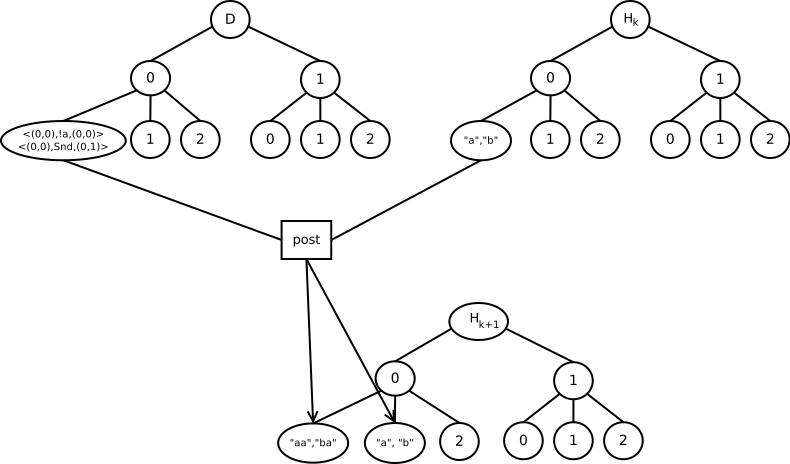
\includegraphics[width=400pt] {bilder/applyrule.png}
\caption{This picture shows the process of applying rules. For each control-state, each rules with that state are applied on each configuration with the same state. This will generate new configurations, not necessarily with the same control-state. For clarity.  tree structure is used to illustrate a hashmap.}
\label{applyrule}
\end{figure}



\subsection{Advantages of Partitioning}
Having partitioned the set $X$ of configurations into a hashmap of $X_k$ of sets, all set operations are made more effective. In a best-case scenario, there would be approximately the same number of configurations for every state in the system. The complexity of checking whether $\alpha_k(c)$ $\in$ $V$ is reduced to $O(log (n/|S|))$ where $S$ is the set of control-states in the system. The complexity of inserting an element is naturally the same.

Additionally, the complexity of calculating the set of post-images of a set $\gamma_k^{k+1}(X)$ is reduced, as we need not perform the calculation of each each $\rho = (s, op, s') \in \delta$ on each $c \in \gamma_k^{k+1}(X)$, but only on the subset of configurations for which $state(c) = s$.


\begin{algorithm}
  \caption{The verification algorithm from section \ref{alg1} in somewhat higher detail. This version includes }\label{euclid}
  \begin{algorithmic}[1]
    \State \textbf{Gamma (V, Seen):}
    \State \hspace{6 mm} con' := concretizations (V)
    \State \hspace{6 mm} con  := c | c $\in$ con $\land$ c $\notin$ Seen
    \\
    \State \textbf{Step (Con, Rules):}
    \For {state $\in$ nodes(V)}
    \State \hspace{6 mm} S := r(c) | $\forall$ c $\in$ con(state) $\land$ $\forall$ r $\in$ Rules(state)
    \EndFor
    \\
    \State \textbf{Alpha (V, S):}
    \State \hspace{6 mm} V:= V $\cup$ views(C)
    \\
    \State \textbf{Verifier (V, Rules, Bad):}
    \For{\texttt{$True$}}
        \If {$\mathcal{R}_k$ $\cap$ $Bad$ $\neq$ $\emptyset$}
        \State return Unsafe
        \EndIf
        \State V := $\mu Alpha(Step(Gamma(V)))$
        \If {$\gamma_k(V)$ $\cap$ $Bad$ = $\emptyset$}
        \State return Safe
        \EndIf
        \State k := k+1
      \EndFor
\end{algorithmic}
\end{algorithm}



\newpage
\section{Final Implementation}
An efficient algorithm in this context is largely an algorithm that avoids performing unnecessary calculations. This can either be done by avoiding to create unnecessary configurations such as was done with the rule hashmap above or by avoiding re-calculating previously calculated results. The algorithm as described above reproduces its steps each iteration; if a configuration \e{c} can be extended to a concretization \e{con} at any point in the verification process, then \e{con} can and will be created in every following iteration. This includes checking whether \e{$\alpha_k(con) \subset V$}, applying a set of rules to the configuration and then adding all the views of the resulting configurations to the set. Each time the calculations are performed, the result will be duplicates and no new views are added to the system.

We solve this by maintaining another hashmap, \e{seen}, of configurations in parallell, containing exactly those concretization that have been accepted. If a configuration \e{c} can be extended to the concretization \e{con}, then we first check if \e{con} is an element of seen. If it is, we discard \e{con}, otherwise we add \e{con} to \e{seen} and also to the set of concretizations to be evaluated in this iteration.

Yet another source of repetition is the fact that there are multiple ways to create the same channel evaluations. Therefore, after a rule has been applied to a concretization, it may result in a configuration already in the set. Instead of performing the costly $\alpha$-calculation, we first check if the newly created configuration is not in fact a duplicate by checking if it is already in \e{V}. If so, the configuration can again be discarded.

The final algorithm amounts to the following pseudo-code representation:

\subsection{Reachability Analysis}
An important step of the verification process which has yet to be covered is that of performing a reachability analaysis, in order to find bad states, if any such states are reachable and find a minimal bad trace leading up to the bad state. See sections \ref{bad} and \ref{traces} for formal definitions of bad states and traces respectively.

Below, a simple technique of finding a minimal bad trace is presented, accompanied with a proof that the trace is in fact minimal.

\subparagraph{Finding Minimal Traces}
When running the verification, if a bad state is found we want to produce a trace leading up to the bad state. Preferably, this would be a minimal trace that leads to the bad state.

The proposed verification method generates a finite set of reachable states (nodes in this context), but it does not record the available transitions between the nodes (i.e. the edges). It is possible to for each node \e{n} to save all nodes \e{n} from which an edge to \e{n'} exists, and thus build the complete reachability graph of the problem. There exists efficient algorithms to solve such a problem, e.g. \e{dijkstra shortest path}, or even the shortest path between any two nodes, e.g. flow-network techniques. Although these algorithms are efficient, building the complete reachability graph would be costly in terms of memory space, as the number of edges may be much larger than the number of states.


We show that due to the method of iteratively constructing the graph, nodes are created in such a way, that if a node $n_{i}$ created in the \e{i}:th iteration is reached by a node $n_{i-1}$ over an edge $e_{i-1}$, the shortest path from the initial node $n_0$ will necessarily be a path $e_1...e_{i-1}$.

\e{Proof.} This is proven using an induction proof. We hypothesize that, if at the point of creation of $n_i$, choosing the parent node $n_{i-1}$ from which an edge $e_{i-1}$ can be taken $n_i$, the path $e_1..e_{i}$ will be the shortest path to $n_i$ and has length \e{i}. Note that the node $n_{i-1}$ must have been created in the previous iteration; had it been created earlier, the edge $e_i$ could have been taken in a previous iteration, and so $n_{i+1}$ would already be a node in the tree.

The base case is that for any node reachable from $n_0$ over any edge $e_0$, $e_0$ will be the shortest path and has length 1. This is trivially true.

Now suppose a node $n_{i+1}$ is reachable over an edge $e_i$ from a node $n_i$, and the node $n_{i+1}$ is not yet in the system. The induction hypothesis states that the path $e_1...e_i$ is the shortest path leading up to $n_i$. If $e_0..e_{i-1}e_i$ would not be the shortest path to $n_{i+1}$, there would be a path $e'_0..e'_{k-1}$ to another node $n_k$ with k < i from which $n_{i+1}$ can be reached. But any such node would have been created in the \e{k}:th iteration of the algorithm, which would contradict the fact that the node $n_{i+1}$ was not already in the system.

Having shown this, we need only record the information of a single parent of a node, in order to build up a tree from which the shortest path from $n_0$ to any node in the system can efficiently be found.


\subsection{Specification Language}
\label{speclang}
In order for the verification algorithm to be easily used, a specification language is needed in which algorithms can be formally defined. We expect such a specification language to

\begin{itemize}
\item
be expressive enough to express all algorithms that are in the scope of the verification program
\item
be independent of the internal representations of the verifier and to demand as little knowledge of the actual verification process as possible from the user
\item
to be as clear as possible in order to ensure that the model at hand in fact corresponds to the actual algorithm, the way it was intended
\end{itemize}

The specification language used is an adaption of previous works in \cite{mpass}. The language simply uses XML to describe an algorithm. There are minor differences between the specification language used here, with respect to that used in by the MPass verification algorithm, and correspond to different expressivness of the models. More specifically, the MPass verifier allows for joint reception and transmission transitions, i.e. a single transition may read a message from a channel and write a message to a channel at the same time. On the other hand, it does not allow for synchronized transitions, this has therefore been added to the language.

\subsubsection{Example}
We return yet again to the Alternating Bit Protocol to examplify the specification language. Bearing in mind the formal definition in section \ref{CS}, a model needs a set of messages, channels, actions and transitions.

We begin by specifying a new protocol, it's name and that it is operating on FIFO buffers. We then specify a set of messages, a set of channels and a set of actions in a similar manner.

\lstset{language=XML}
\begin{lstlisting}[frame=single]
<protocol name="Alternating Bit Protocol" medium="FIFO>
<messages>
      <message>ack0</message>
      <message>ack1</message>
      <message>mesg0</message>
      <message>mesg1</message>
</messages>

<channels>
      <channel>c1</channel>
      <channel>c2</channel>
</channels>

<actions>
      <action>Rcv</action>
      <action>Snd</action>
</actions>
\end{lstlisting}

We then continue by defining the different processes in the system, i.e. the sender, receiver and observer. Such a process is defined by its states and its transitions. In the specification language, we differentiate between transitions over an action, and transitions that modify a channel. The latter type is called a \e{rule} in the specification language, in order to comply with the names used in the MPass specification language. This should not be confused with the word as used earlier in this section.

\begin{lstlisting}[frame=single]
  <role name="SENDER">
    <states>
      <state type="initial">Q0</state>
      <state>Q1</state>
      <state>Q2</state>
      <state>Q3</state>
    </states>
    <action>
        <current_state>Q0</current_state>
        <type>Snd</type>
        <next_state>Q1</next_state>
    </action>
    <rule>
        <current_state>Q1</current_state>
        <send_message>mesg0</send_message>
        <next_state>Q1</next_state>
        <channel>c1</channel>
    </rule>
\end{lstlisting}

Last, we specify that the processes \texttt{SENDER} and \texttt{OBSERVER}, and  \texttt{RECEIVER} and \texttt{OBSERVER} are to be synchronized over the actions \texttt{Snd} and \texttt{Rcv} respectively.

\begin{lstlisting}[frame=single]
<synchronize>
        <first_role>SENDER</first_role>
        <second_role>OBSERVER</second_role>
        <action>Snd</action>
</synchronize>
<synchronize>
        <first_role>RECEIVER</first_role>
        <second_role>OBSERVER</second_role>
        <action>Rcv</action>
</synchronize>
\end{lstlisting}

\section{Related Work}
%Early model checking consisted of mathematically proving correctness, by manual inspection. As this is a cumbersome and error-prone task, much research effors were put in to the automatication of the process\cite{emerson2008}.

%The field first gaind ground with ground breaking work of Pnueli, being the first to suggest the use of \e{temporal logic} to analyse concurrent programs\cite{pnueli1977}. To this end, Pnueli formulated a small set of linear temporal operators, from which LTL-formulas could be formulated with high expressivness. As opposed to linear time logic in which assersions can be made on an execution path, \e{branching time logic} allows for assrsion to be set with respect to all possible future paths. Although several formulations exists, the most widely used is CTL (Computation Tree Logic), as suggested by Clarke and Emerson\cite{emerson1980}. These intitial efforts continue to be researched and extended today, notable is for example timed CTL which allows verification of systems with real-time constraints. A multitude of sophisticated and efficient implementations exists for these logics, well known examples are SPIN\cite{spin}, NuSMV\cite{nusmv} and UPPAAL\cite{uppaal} for LTL, CTL and tCTL respectively.

%Temportal model checking provides effiecient (polynomial or linear) algorithms for verification, but struggles with the much researched state space explosion\cite{clarke2012}. Building upon CTL logic, \e{symbolic model checking} attempts to reduce the state space growth representing states as order binary decision diagrams (OBDDs)\ref{nr 70 in book, Bryant} which may, but are not guaranteed tp, greatly reduce the number of states in the representation. More recent symbolic representations have focused on expressing functions in conjunctive normal form, CNF, thus allowing SAT techniques to be used to perform quantifier elimination.\cite{mcmillan}\todo{find ref, MPass?} 

%Symbolic model checking is useful when the system under observation has a large number of states, for example the verification of a piece of hardware. 

%Regular model checking:
%\cite{boigelot2003}\cite{resten1997}

\e{Parameterized model checking} focuses verification scenarious where the size of the problem under observation is a parameter of the system, and the size has no trivial upper bound. The goal is to verify the correctness of the system regardless of the value of the parameter. As this generally corresponds to a transition system of infinite size, research in this field of verification focuses on techniques to limit the size of the transition system.

On such method is the \e{invisible invariants} method\cite{invinv}, which similar to \cite{parosh} and \cite{namjoshi} use \e{cut-off} points to check invariants. Such cut-off points can be found dynamicly\cite{kaiser2010} or be constant\cite{emerson1995}. The works of Namjoshi\cite{namjoshi}  show that methods based on process invariants or cut-offs are complete for safety properties.

Small model systems have been investigated in \cite{kaiser2010}, which combines it with ininite state backward coverability analysis. Such methods prevent its use on undecidable reachability problems, such as those considered in \cite{parosh}. The work of \cite{parosh} also show that the problem is decidable for a large class of well quasi-ordered systems, including Petri Nets\cite{parosh}. Practical results indicate that these methods may be decidable for yet larger classes of systems. More on well-structured infinite transition systems can be found in \cite{finkel2001}.

Abstract interpretation techniques were first described by Cousot and Cousot\cite{cousot1977}\cite{cousot1979}. Similar work to \cite{parosh} can be found in \cite{raskin2006, ganty2006}.

% Modelchecking boken, sida 81 påstår att dijkstra var först.
Edsger Dijkstra was the first to consider the interaction between processes communicating over channels\cite{dijkstra1972}\cite{baier2008}. In \cite{bz83}, the authors show that verification of perfect channels systems is undecidable, by relating it to the simulation of a Turing Machine\cite{bz83}. The decidability of lossy channels has been researched in\cite{287591, gordon}.


% Part on other attempts to solve the same problem
Similar to this thesis, \cite{le2006} make use of abstract interpretation to channel systems, applying the technique to regular model checking. MPass\cite{mpass} is a verification tool for channel systems, that restates the verification problem to an equivalent first-order logic, which is then solved by an SMT solver. Its input language is roughly the same as this thesis, although the tool is more general, being applicable also on \e{stuttering} and unordered channels.



\bibliographystyle{ieeetr} 
\bibliography{references}



\end{document}
